\documentclass{article}

% Package necessari
\usepackage[a4paper]{geometry}
\usepackage[utf8]{inputenc}
\usepackage[italian]{babel}
\usepackage[T1]{fontenc}
\usepackage{amsmath}
\usepackage{amssymb}
\usepackage{graphicx}
\usepackage[table, dvipsnames]{xcolor}
\usepackage{listings}
\usepackage{hyperref}
\usepackage{enumitem}
\usepackage{fancyhdr}
\usepackage{algorithm}
\usepackage[noend]{algpseudocode}

% Impostazione delle lunghezze di alcuni elementi del documento
\setlength{\parskip}{1em}
\setlength{\parindent}{0em}
\setlength{\arrayrulewidth}{0.1em}

% Informazioni per la title page
\title{\small{Corso di Performance Modeling of Computer Systems \& Networks} \\
\huge{Studio delle prestazioni di un Ufficio Postale di \\
\textbf{Poste Italiane}}}

\date{A.A. 2020/2021}

\author{A. Chillotti\thanks{\texttt{\href{mailto:alessandro.chillotti@outlook.it}{alessandro.chillotti@outlook.it}}}
\and 
C. Cuffaro\thanks{\texttt{\href{mailto:cristiano.cuffaro@outlook.com}{cristiano.cuffaro@outlook.com}}} 
\and 
S. Tiberi\thanks{\texttt{\href{mailto:simone.tiberi.98@gmail.com}{simone.tiberi.98@gmail.com}}}
}

% Impostazione del package hyperref
\hypersetup{
    colorlinks=true,
    linktocpage=true,
    linkcolor=blue,
    urlcolor=blue,
    pdftitle={Studio delle prestazioni di un Ufficio Postale di Poste Italiane},
    pdfauthor={A. Chillotti, C. Cuffaro e S. Tiberi},
}

% Colori per i listing
\definecolor{code_red}{rgb}{0.6,0,0} % strings
\definecolor{code_green}{rgb}{0.25,0.5,0.35} % comments
\definecolor{code_purple}{rgb}{0.5,0,0.35} % keywords
\definecolor{code_background}{rgb}{0.95,0.95,0.92} % background

% Altri colori
\definecolor{forestgreen}{rgb}{0.13, 0.55, 0.13}
\definecolor{airforceblue}{rgb}{0.36, 0.54, 0.66}
 
% Stile del codice standard (C)
\lstset{
	language=C, 
	backgroundcolor=\color{code_background},
	frame=single,
	basicstyle=\ttfamily,
	keywordstyle=\color{code_purple}\bfseries,
	stringstyle=\color{code_red},
	commentstyle=\color{code_green},
	numbers=left,
	numberstyle=\small\color{gray},
	numbersep=5pt,
	tabsize=4,
	showtabs=false,
	showspaces=false,
	showstringspaces=false,
	escapechar=|, 
	captionpos=b,
	breaklines=true,
}

\pagestyle{fancy}
\fancyhf{}
\lhead{\small A.Chillotti, C. Cuffaro, S. Tiberi}
\rhead{\small Performance Modeling of Computer Systems \& Networks}
\cfoot{\thepage}
%\cfoot{Pagina \thepage}

% Spaziatura tabelle
\renewcommand{\arraystretch}{1.5}

\graphicspath{ {./figs/} }
% Definizione del colore delle tabelle
\newcommand{\tablecolors}[1][2]{\rowcolors{#1}{yellow!50}{yellow!25}}

% Definizione dello stile da usare per la P di probabilità (grassetto in math-mode)
\newcommand{\pr}{\mathbf{P}}

% Forzatura del displaystyle in math-mode
\everymath\expandafter{\the\everymath\displaystyle}

\newcommand{\scaption}[1]{\caption{\small{#1}}}

\newcommand{\uo}{\textsl{Unica Operazione}}
\newcommand{\pp}{\textsl{Pagamenti \& Prelievi}}
\newcommand{\sr}{\textsl{Spedizioni \& Ritiri}}

\begin{document}
\maketitle

\section{Presentazione del caso di studio}
Il sistema oggetto dell'analisi in questione eroga le seguenti tipologie di servizi:
\begin{enumerate}
\item \textbf{Unica Operazione} (e.g. ricarica \textsl{PostePay}, invio raccomandata e pagamento di massimo 3 bollettini)
\item \textbf{Pagamenti \& Prelievi} (e.g. pagamento di un numero arbitrario di bollettini, bollo auto e libretti)  
\item \textbf{Spedizioni \& Ritiri} (e.g. invio corrispondenza, lettere, pacchi e raccomandate)
\end{enumerate}

Per essere serviti i clienti possono:
\begin{itemize}
\item Recarsi all'ufficio postale, prendere un ticket relativo al servizio a cui sono interessati e mettersi in coda in attesa del proprio turno. Nel caso in cui essi dimostrano di essere titolari di un conto \textsl{BancoPosta} potranno accodarsi in una fila dedicata.
\item Prenotare un ticket mediante l'applicazione \textsl{"Ufficio Postale"} per una determinata fascia oraria, al fine di essere serviti dal primo sportello disponibile entro 40 minuti, ma non prima, dall'orario di prenotazione.
\end{itemize}

Un insieme di sportelli serve le richieste degli utenti in accordo alle seguenti regole: 
\begin{enumerate}[label=R\arabic*)]
\item I clienti titolari di un conto \textsl{BancoPosta} vengono serviti con una priorità maggiore rispetto agli altri, indipendentemente dal ticket scelto.
\item Poiché, per definizione, ticket di tipo \textbf{Unica Operazione} dovrebbero richiedere meno tempo per essere processati, viene assegnata loro la massima priorità
\item I ticket di tipo \textbf{Spedizioni \& Ritiri} vengono serviti da uno sportello dedicato il quale, in assenza di questa tipologia di ticket, opera come gli altri. Il comportamento di tale servente è schematizzato in figura \ref{fig:presentazione-1}. 
\end{enumerate}

\begin{figure}[ht]
\centering
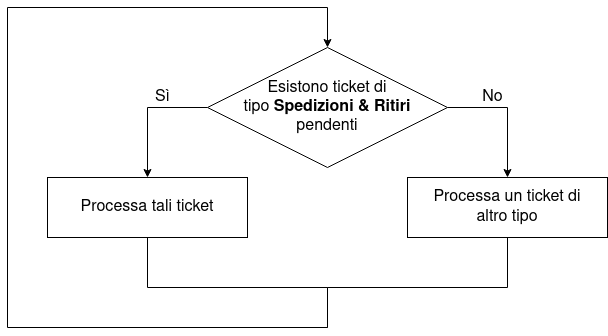
\includegraphics[width=0.75\linewidth]{presentazione-1}
\scaption{Schema del comportamento del servente dedicato ai ticket di tipo \textbf{Spedizioni \& Ritiri}}
\label{fig:presentazione-1}
\end{figure}
\section{Obiettivi dello studio}
L'obiettivo dello studio è quello di individuare ed analizzare gli indici prestazionali del sistema \textbf{Poste Italiane} e di proporre una miglioria nel sistema di processamento delle richieste, al fine di ridurre il tempo medio d'attesa sperimentato dai clienti in coda.
\chapter{Modello concettuale}\label{chp:modello-concettuale}
\begin{figure}[ht]
\centering
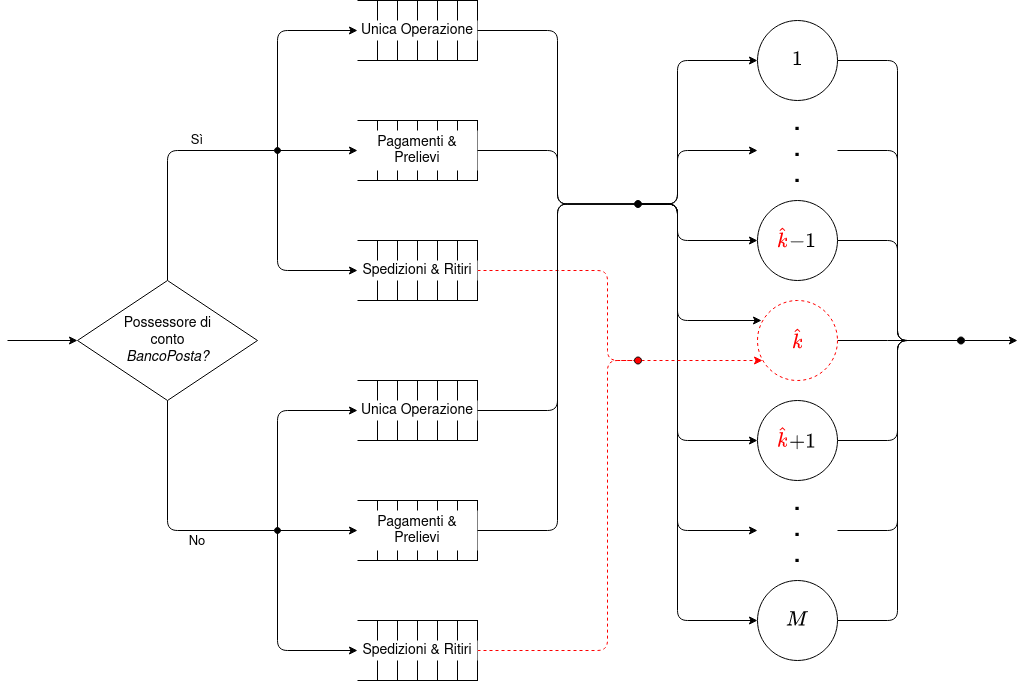
\includegraphics[width=\linewidth]{modello-concettuale-1}
\caption{Diagramma del sistema \textbf{Poste Italiane}}
\label{fig:modello-concettuale-1}
\end{figure}

Il funzionamento del sistema è illustrato dal diagramma in figura \ref{fig:modello-concettuale-1}. Di seguito è riportata una descrizione degli elementi in esso utilizzati:
\begin{itemize}
\item Il rombo rappresenta un meccanismo di ripartizione del flusso in ingresso nelle opportune code, a seconda della titolarità o meno di un conto \textsl{BancoPosta} da parte dei clienti.
\item Ciascuna coda modella una fila di clienti possessori dello stesso tipo di ticket.
\item Ciascun servente rappresenta uno sportello dell'ufficio postale
\begin{itemize}
\item Il $\ded$-esimo servente (evidenziato in {\color{red} rosso}) rappresenta lo sportello dedicato per la gestione dei ticket di tipo \sr{}, il cui comportamento è stato già illustrato nel flow chart in figura \ref{fig:presentazione-1}.
\end{itemize}
\end{itemize}

Ad ogni istante di tempo, lo stato del sistema è univocamente determinato dai valori assunti dalle seguenti $M + 12$ variabili di stato:
\begin{itemize}
\item Per ciascuno degli $M$ sportelli si ha:
\begin{equation}
Server_r \in
\left\lbrace \mathtt{IDLE},\ \mathtt{BUSY} \right\rbrace
\end{equation}
con $r \in \lbrace 1, 2, \dots, M \rbrace$.
\item Per ciascuna delle 6 classi di utenza:
\begin{itemize}
\item Il numero totale di clienti della $c-$esima è modellato dalla variabile $Customers_{c}$
\item Il numero di clienti in servizio della $c-$esima è modellato dalla variabile $InService_{c}$
\end{itemize}
con $c$ appartenente a:
\begin{multicols}{2}
\begin{itemize}
\item \uo{} \textsl{BancoPosta}
\item \pp{} \textsl{BancoPosta}
\item \sr{} \textsl{BancoPosta}
\item \uo{} \textsl{Standard}
\item \pp{} \textsl{Standard}
\item \sr{} \textsl{Standard}
\end{itemize}
\end{multicols}
\end{itemize}

Infine, si assume che:
\begin{itemize}
\item I clienti abbiano un comportamento di tipo \textsl{one-step}\footnote{Avere un comportamento di tipo \textsl{one-step} significa che vi può essere, ad ogni istante di tempo, lo spostamento di un solo cliente alla volta.}.
\item Non è possibile avere uno sportello libero se in coda è presente almeno un cliente con ticket processabile da tale sportello (sistema \textsl{work conserving}\footnote{La proprietà di \textsl{work conserving} è valida entro i vincoli imposti dal caso di studio.}).
\item All'inizio ed alla fine del periodo d'osservazione lo stato del sistema è il seguente:
\begin{equation}
\begin{cases}
Server_r =\mathtt{IDLE} & \forall\ r \\[1em]
Customers_{c} = \mathtt{NONE} & \forall\ c \\[1em]
InService_{c} = \mathtt{NONE} & \forall\ c
\end{cases}
\end{equation}
\end{itemize}
\chapter{Modello delle Specifiche}\label{chp:modello-specifiche}
Le seguenti variabili matematiche, definite per ogni istante di tempo $t$, identificano univocamente una rappresentazione a livello delle specifiche dello stato del sistema:

\begin{itemize}
\item Lo stato dello sportello $r$-esimo è dato da:
\begin{equation}
\label{eqn:modello-specifiche-3}
Server_r(t) \in \lbrace 0, 1 \rbrace
\end{equation}
\item Per ciascuna classe $c$ il numero totale di clienti è definito come:
\begin{equation}
\label{eqn:modello-specifiche-2}
Customers_c(t) \in \mathbb{N}
\end{equation}
\item Per ciascuna classe $c$ il numero di clienti in servizio è definito come segue:
\begin{itemize}
\item Per $c$ diversa da \sr{} \textsl{BancoPosta} e \sr{} \textsl{Standard}:
\begin{equation}
\label{eqn:modello-specifiche-2}
InService_c(t) \in \lbrace 0, 1, \dots, M \rbrace
\end{equation}
\item Altrimenti:
\begin{equation}
\label{eqn:modello-specifiche-2}
InService_c(t) \in \lbrace 0, 1 \rbrace
\end{equation}
\end{itemize}
\end{itemize}

Dalle variabili appena descritte, è immediato ricavare il numero di clienti in coda per ciascuna classe di utenza $c$:
\begin{equation}
Queue_c(t) = Customers_c(t) - InService_c(t)
\end{equation}

Di seguito sono riportate alcune assunzioni che saranno alla base di questa e delle successive fasi dello studio:
\begin{itemize}
\item I clienti arrivano all'ufficio postale ad istanti di tempo casuali, il che implica:
\begin{itemize}
\item Distribuzione poissoniana degli arrivi.
\item Distribuzione esponenziale dei tempi di interarrivo.
\end{itemize}
\item La probabilità che un cliente sia titolare di un conto \textsl{BancoPosta} è pari a $p_{BP} = 0.25$.
\item Le probabilità con cui ciascuna tipologia di ticket viene acquisita sono le seguenti:
\begin{equation*}
\begin{array}{l c l}
\uo{} & \rightarrow & p_{UO} = 0.5 \\
\pp{} & \rightarrow & p_{PP} = 0.35 \\
\sr{} & \rightarrow & p_{SR} = 0.15
\end{array}
\end{equation*} 
\item I tempi di servizio sono distribuiti esponenzialmente.
\item I clienti afferenti ad una stessa coda vengono serviti in accordo ad una disciplina FIFO (First-In, First-Out).
\item Il servizio di un cliente non può essere interrotto per favorire l'avanzamento di un altro con priorità superiore.
\end{itemize}

Al fine di agevolare la comprensione del funzionamento dello scheduler di sistema, di seguito sono riportati gli pseudocodici \ref{alg:modello-specifiche-1} e \ref{alg:modello-specifiche-2} che descrivono, rispettivamente, il comportamento del servente generico e di quello dedicato.

\begin{algorithm}[ht]
\SetAlgoLined
\While{true}{
	\uIf{`\uo{} \textsl{BancoPosta}' queue not empty}{
		\textit{processes the first ticket of that type}\;
	}
	\uElseIf{`\pp{} \textsl{BancoPosta}' queue not empty}{
		\textit{processes the first ticket of that type}\;
	}
	\uElseIf{`\uo{} \textsl{Standard}' queue not empty}{
		\textit{processes the first ticket of that type}\;
	}
	\uElseIf{`\pp{} \textsl{Standard}' queue not empty}{
		\textit{processes the first ticket of that type}\;
	}
	\uElse{
		\textit{do nothing}\;
	}
}
\caption{Algoritmo di schedulazione del servente generico}
\label{alg:modello-specifiche-1}
\end{algorithm}

\begin{algorithm}
\SetAlgoLined
\While{true}{
	\uIf{`\sr{} \textsl{BancoPosta}' queue not empty}{
		\textit{processes the first ticket of that type}\;
	}
	\uElseIf{`\sr{} \textsl{Standard}' queue not empty}{
		\textit{processes the first ticket of that type}\;
	}
	\uElseIf{`\uo{} \textsl{BancoPosta}' queue not empty}{
		\textit{processes the first ticket of that type}\;
	}
	\uElseIf{`\pp{} \textsl{BancoPosta}' queue not empty}{
		\textit{processes the first ticket of that type}\;
	}
	\uElseIf{`\uo{} \textsl{Standard}' queue not empty}{
		\textit{processes the first ticket of that type}\;
	}
	\uElseIf{`\pp{} \textsl{Standard}' queue not empty}{
		\textit{processes the first ticket of that type}\;
	}
	\uElse{
		\textit{do nothing}\;
	}
}
\caption{Algoritmo di schedulazione del servente dedicato}
\label{alg:modello-specifiche-2}
\end{algorithm}

\newpage
In tabella \ref{table:modello-specifiche-1} sono riportati tempi di servizio medi assunti per ciascuna tipologia di ticket, sperimentati su un singolo servente.
\begin{table}[ht]
\centering
{\tablecolors
\begin{tabular}{| l | r |}
\hline
Tipologia di ticket & Tempo di servizio medio \\
\hline
\uo{} & 7 min \\
\hline
\pp{} & 14 min \\
\hline
\sr{} & 10 min \\
\hline
\end{tabular}}
\caption{Assunzioni sui tempi medi di servizio sul singolo sportello}
\label{table:modello-specifiche-1}
\end{table}	

\begin{table}[ht]
\centering
{\tablecolors
\begin{tabular}{| l | r |}
\hline
Grandezza & Valore misurato nel 2018 \\
\hline
N$^o$ di clienti al giorno & 1.5 mln \\
\hline
N$^o$ di uffici postali & 12 812 \\
\hline
\end{tabular}}
\caption{Estratto dei dati di interesse a partire dalla fonte citata}
\label{table:modello-specifiche-2}
\end{table}

Per stimare il throughput dell'intero sistema si è fatto uso dei dati dati provenienti da \textsl{"Principali dati economici e finanziari di Poste Italiane"}\footnote{\url{https://www.posteitaliane.it/it/performance-finanziaria.html}} nel modo seguente:
\begin{equation}
X = \frac{\# \text{clienti al giorno}}{\#\text{uffici postali}} = \frac{1500000}{12812}\ req/wd = \frac{1500000}{12812\cdot 480} \simeq 0.243912\ req/min
\end{equation} 
dove la conversione da giornata lavorativa (\textsl{wd}) a minuti effettivi di lavoro è stata realizzata dividendo per il solo periodo d'erogazione dei ticket. Il motivo è che quest'ultimo ha un'ampiezza fissa, mentre quella del tempo di smaltimento è funzione delle richieste pendenti (cap. \ref{chp:presentazione}). In definitiva, poiché si divide per un numero più piccolo, si effettua una stima per eccesso.

È opportuno osservare che, sotto l'ipotesi di \textsl{job flow balance}, la frequenza d'arrivo media al centro $\lambda$ coincide con il throughput $X$.



\end{document}